% Copyright (C) 2012 Davidlohr Bueso <dave@gnu.org>

% STATE OF THE ART
\section{Fdisk's State of the Art}
\subsection{Fdisk Problems}
\subsubsection{Smelly, Legacy Code}

\begin{frame}\frametitle{Smelly, Legacy Code}
  \begin{columns}
    \begin{column}{.5\linewidth}
      The Linux fdisk program is over 20 years old and is a complex product of multiple authors, concepts, specifications and coding styles, among others.\newline

      As a result, code is \textbf{glued} together, and making it difficult and error prone to enhance and fix bugs.
    \end{column}
    \begin{column}{.5\linewidth}
      
\includegraphics[scale=0.2]{img/glustick}
    \end{column}
  \end{columns}
\end{frame}

\begin{frame}\frametitle{Smelly, Legacy Code}
\begin{figure}
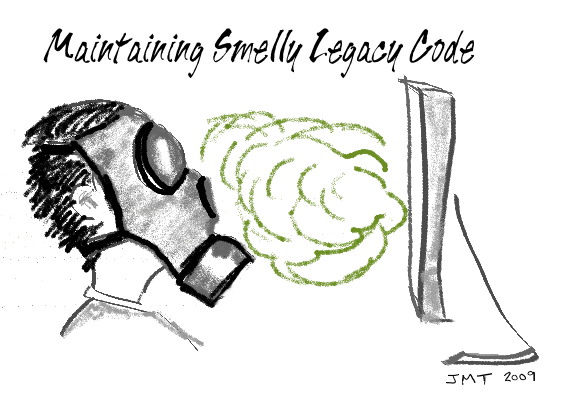
\includegraphics[scale=0.4]{img/SmellyLegacyCode}
\end{figure}
\end{frame}

\subsubsection{Stuck in the Past}
\begin{frame}\frametitle{Stuck in the Past}
  \begin{columns}
    \begin{column}{.5\linewidth}
      
\includegraphics[scale=0.3]{img/linkman}
       \end{column}
    \begin{column}{.5\linewidth}
      \begin{itemize}
      \item DOS compatibility mode
      \item Doesn't work with GPT
      \item CHS addressing
      \item Mainframe style UIs\newline
      \end{itemize}
    \end{column}
  \end{columns}
\end{frame}

\subsubsection{Everyone Looses}
\begin{frame}\frametitle{Everyone Looses}
  \begin{columns}
    \begin{column}{.5\linewidth}
      \begin{block}{Hackers loose}
        Adding new code and extending functionality is difficult, tedious and error prone.
      \end{block}
      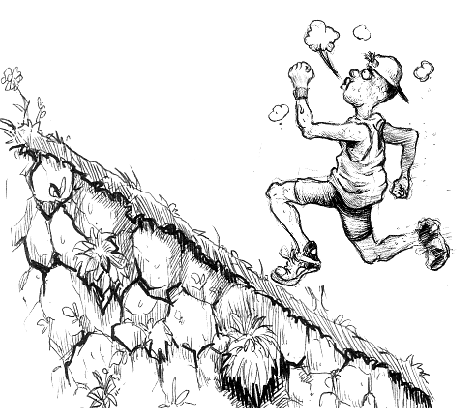
\includegraphics[scale=0.3]{img/running-uphill}
    \end{column}
    \begin{column}{.5\linewidth}
      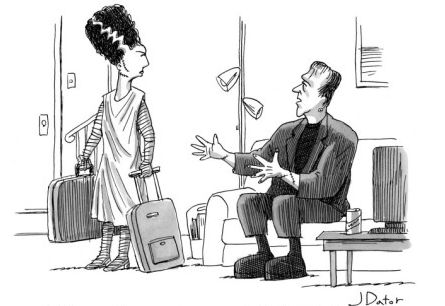
\includegraphics[scale=0.5]{img/leaving}
      \begin{block}{Users loose}
        Fdisk \textbf{cannot} compete with other partitioning tools and thus looses users. Hey, healthy competition is good for everyone!
      \end{block}
    \end{column}
  \end{columns}
\end{frame}

\subsection{Fixing Fdisk}
\begin{frame}
  \begin{block}{Fixing this mess}
    Update fdisk to modern, XXI century, disk standards.
  \end{block}
\end{frame}

\begin{frame}\frametitle{Short Term}
  Short term goals:
  \begin{itemize}
  \item Cleanup and refactor current, legacy, code
  \item Create an internal API that abstracts disklabel concepts and specifications
  \item Add GUID Partition Table (GPT) support
  \end{itemize}
\end{frame}

\begin{frame}\frametitle{Longer Term}
  Long term goals:
  \begin{itemize}
  \item Create an independent, libfdisk shared library.
  \item Rewrite cfdisk and sfdisk with new library.
  \end{itemize}
\end{frame}

\begin{frame}
  \begin{block}{Caveats}
    \begin{itemize}
    \item Changes must maintain backwards compatibility.
    \item Write high quality code that's maintainable, at least for the next few decades.
    \end{itemize}
  \end{block}
\end{frame}
